\graphicspath{ {mainmatter/Berdahl_2011/} }
\title*{2011: Satellite CCRMA: A Musical Interaction and Sound Synthesis Platform}
 \titlerunning{A Musical Interaction and Sound Synthesis Platform} 
\author{Edgar Berdahl and Wendy Ju}
\authorrunning{Berdahl and Ju}
% Use \authorrunning{Short Title} for an abbreviated version of
% your contribution title if the original one is too long
%\institute{Name of First Author \at Name, Address of Institute, \email{name@email.address}
%\and Name of Second Author \at Name, Address of Institute \email{name@email.address}}
%
%
\maketitle


\abstract*{This paper describes a new Beagle Board-based platform for teaching and practicing interaction design for musical applications. The migration from desktop and laptop computer-based sound synthesis to a compact and integrated control, computation and sound generation platform has enormous potential to widen the range of computer music instruments and installations that can be designed, and improves the portability, autonomy, extensibility and longevity of designed systems. We describe the technical features of the Satellite CCRMA platform and contrast it with personal computer-based systems used in the past as well as emerging smart phone-based platforms. The advantages and trade-offs of the new platform are considered, and some project work is described.
}



%\textbf{{Keywords}}
%Wearable display, sonification, visualisation, user experience, design
%aesthetics, physical computing, multimodal expression, bimodal display

\section{Introduction}

As instructors of CCRMA's course in Physical Interaction Design for Music \cite{Verplank:2001}, we have noticed that many of incredibly novel and innovative musical instruments and installations created in our course over the years have very short lives; even projects demonstrated at the NIME conference \cite{Wilkerson:2002,Shiraiwa:2003,Wilson:2003,Lugo:2005,Carlile:2005,Bowen:2005,Dahl:2007,Schlessinger:2009, Gao:2007} are often inoperable just a year afterwards. Conversations with researchers and musicians at a wide variety of other institutions indicate that this is phenomenom is not isolated to CCRMA alone, and that, even for the very-motivated, it takes enormous effort to keep NIME instruments in a functional and performable state. This lack of longevity and robustness creates a situation where 1) the quality of music produced by NIME instruments is limited by the fact that the instruments do not last long enough for musicians to develop expertise, to compose great scores, or refine the initial instrument designs, and 2) the quality of shared learning from NIME instruments is limited by the fact that the instruments are seldom transfered or built upon except by the same researchers who originated a particular design. While the rapid obsolescence of new musical controllers might be caused by the relatively short attention span of students or by the focus on novelty within the community, we believe that some element of the blame might be placed on the computer platforms that are at the heart of most NIME instruments. 

\begin{figure}[t]
	\centering
		%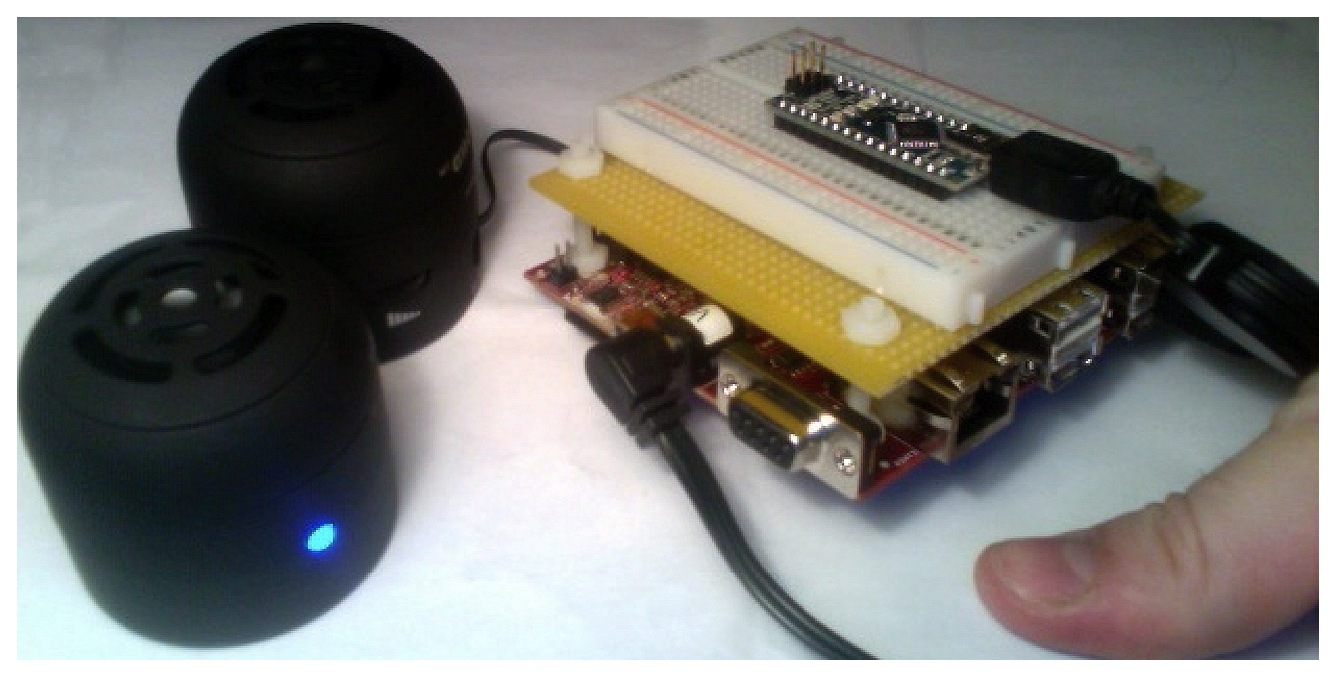
\includegraphics[width=3in]{Photos/SatelliteCCRMA.eps}
		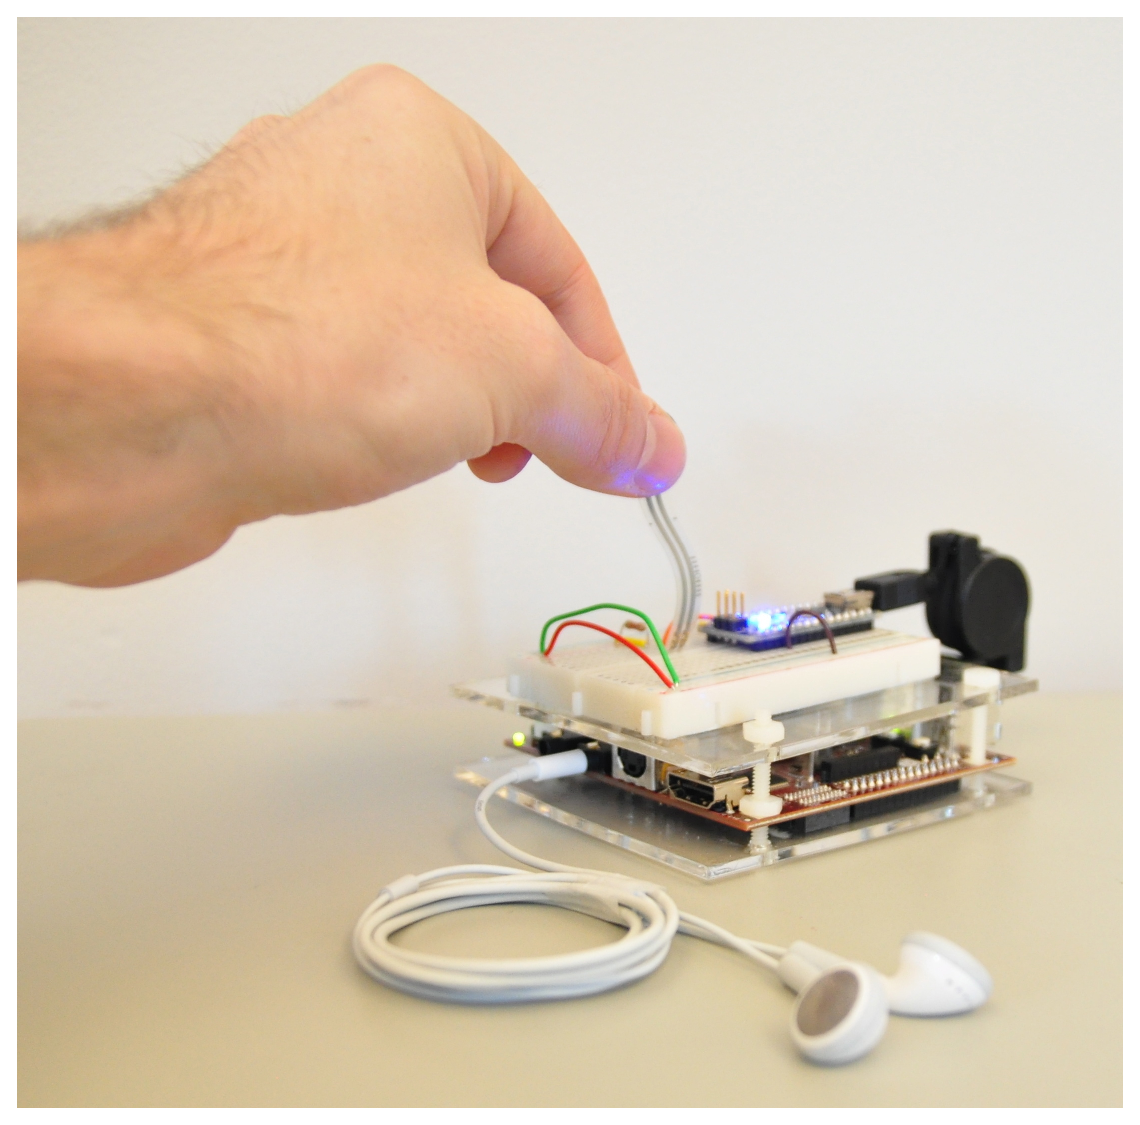
\includegraphics[width=2.7in]{Photos/sat1.eps}
	\caption{Satellite CCRMA}
	\label{Berdahl:fig:Platform}
\end{figure}

Satellite CCRMA (Figure~\ref{Berdahl:fig:Platform}) is a musical interaction design platform designed to support the creation of new instruments for musical expression as well as sound installations. It incorporates a single-board OMAP-based Linux computer, an Arduino-based microcontroller, and a breadboard for electronics prototyping.   By creating a platform which includes a small, inexpensive and autonomous Linux computer, we hope to free NIME designs from the constraints and obstacles associated with platforms which use more general-purpose laptops and desktop workstations.

This paper describes the Satellite CCRMA platform design, its underlying rationale, our initial forays into introducing this platform to students in our Physical Interaction Design for Music course, and what we have learned so far. While it will be many years before we can empirically determine whether our platform is indeed longer-lived than the alternatives, our interim assessments of the affordability, adoptability and the extensibility of the platform give us great optimism that that the platform will be of great use to a large number of people within the NIME community and beyond. 

\section{Platform Description}
\subsection{Hardware}
The Satellite CCRMA platform is centered around the OMAP35x embedded processor line from Texas Instruments, which can run Linux.  We currently use the Beagle Board (see the maroon-colored board in Figure~\ref{Berdahl:fig:Platform}), which features the OMAP3530 processor.  The processor incorporates a superscalar ARM Cortex-A8 core running at 600MHz as well as an a TMS320C64x+ 16-bit fixed-point DSP running at 430MHz.  The Beagle Board connects by way of a USB hub incorporating Ethernet to the Arduino Nano, which is inserted into a solderless breadboard (see Figure~\ref{Berdahl:fig:Platform}, rear).  The following list shows the parts that we used in our initial Satellite CCRMA design with our students during the Autumn quarter in 2010:

\begin{itemize}
\item Beagle Board Rev C4\footnote{\url{http://beagleboard.org/hardware}}
\item Arduino Nano\footnote{\url{http://www.arduino.cc/en/Main/ArduinoBoardNano}}
\item Solderless breadboard
\item 4GB (or larger) SD card 
\item GWC Technology HE2440 USB 2.0 4-Port Hub with Ethernet Adapter
\item Two GT Max adjustable-length USB cables
\item Ethernet cable
\item 2.5A 5V switching power adaptor (For example DVE DSA-15P-05 US)
\end{itemize}

Since this deployment, we have begun moving the platform to the similar Beagle Board XM. Depending on the intensity of the output sound and the loudspeaker size required, we suggest supplementing the kit with compact mobile speakers so that sound production can be localized to the instrument.


\subsection{Software}
We have prepared a special SD card image for the platform that boots Ubuntu Linux into an environment with pre-installed Linux audio applications including the Jack audio server, Pure Data Extended, Faust, JackTrip and ChucK.  Because Satellite CCRMA can easily be connected to the Internet, many new packages can be easily installed (e.g. \texttt{sudo apt-get install lynx}).  Other packages may need to be compiled for the ARM architecture; however, cross-compiling may not be necessary because the SD card installation comes with the gcc tools preinstalled.  The SD card image is especially valuable because we have tested it---otherwise, compiling a new SD card image from scratch can easily require multiple days of work.  For more information on our SD card image and the community we are building for artists, please see the project page. \footnote{\url{https://ccrma.stanford.edu/satellite}}

In our class, we currently have students program their sound synthesis engines using Pure Data Extended.  This graphical environment allows rapid prototyping by connecting together objects using patch cords.  For example, a student can login to his or her Satellite CCRMA kit remotely over Ethernet, load the audio server using the command \texttt{qjackctl \&}, start the audio server, and finally start Pure Data Extended by typing \texttt{pd \&}.  This causes an X-Window to be forwarded over the Ethernet connection, including something similar to the Pure Data Extended patch shown in Figure~\ref{Berdahl:fig:PdPatch}.

\begin{figure}[t]
	\centering
		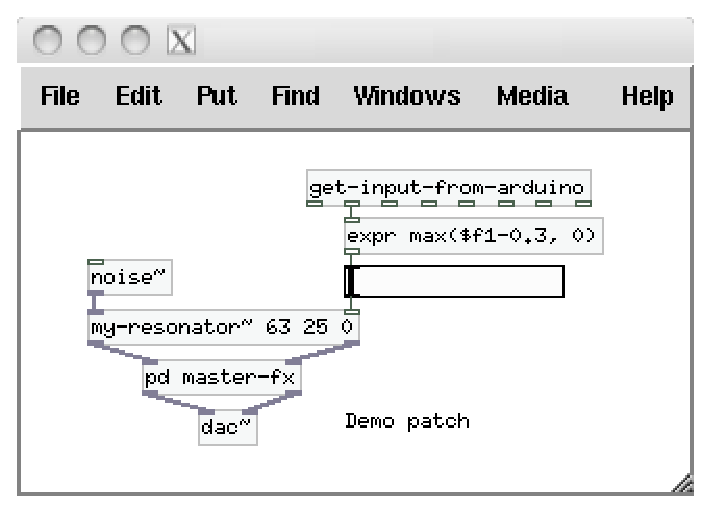
\includegraphics[width=2.9in]{Photos/Demo-Patch.eps}
	\caption{Demonstration patch in Pure Data}
	\label{Berdahl:fig:PdPatch}
\end{figure}

\section{Motivation}


A generic architectural diagram for musical interaction design platform is shown in Figure \ref{Berdahl:fig:architecture}. Although the specific microcontrollers, computer operating systems, hardware, software, firmware, communications protocols, etc used by different members of the NIME community differ, this diagram reflects the fact that most musical interaction platforms use both a microcontroller (to collect and process sensor data, and also to control actuators) and a microprocessor (to perform more computational challenging tasks such as sound synthesis). What we have observed is that the weak link, as far as longevity and robustness are concerned, is the computer housing the microprocessor. Because computers are expensive, people seldom devote separate computers to their NIME designs; instead they use the same machine that they are writing emails and theses on as the critical engine of their new musical instruments. These instruments thus suffer collateral damage every time we upgrade our operating systems, or install a new version of Java, or switch to new hardware.

\begin{figure}[t]
	\centering
		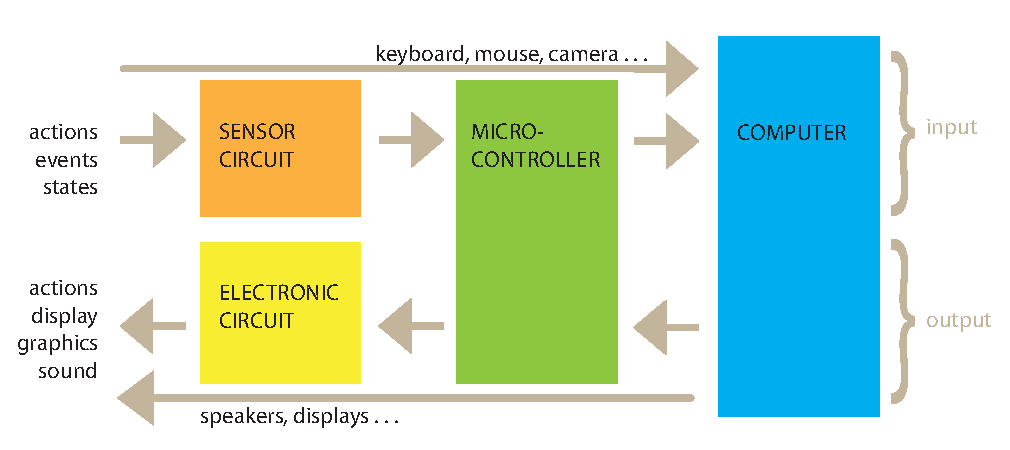
\includegraphics[width=\textwidth]{Photos/PIDplatformarchitecture.eps}
	\caption{Physical Interaction Design Platform Architecture}
	\label{Berdahl:fig:architecture}
\end{figure}

At a base level, any system that we would use in our class would need to be affordable (students balk at paying more than \$150--what they pay for textbooks in a normal class), adoptable (able to be picked up and put to novel use within a school term), and extensible (able to support a wide variety of ideas that we the instructors didn't think of when we gave the students the systems). We also had the following criteria in mind when we were developing the system: 
\subsection{Longevity}
Most acoustic musical instruments stay operable for many years with minimal maintenance.  Hence, as soon as a musician acquires a musical instrument, he or she can often assume that he or she can practice, learn repertoire, compose, and even make adjustments to the instrument for many years to come.  Hence, the \emph{longevity} of an acoustic musical instrument promotes the development of virtuosity.

As we mentioned before, we believe that one of the challenges to longevity in prior music interaction platforms was that they relied on the use of a non-dedicated computer to stay within a reasonable price point. 

\begin{figure}[t]
	\centering
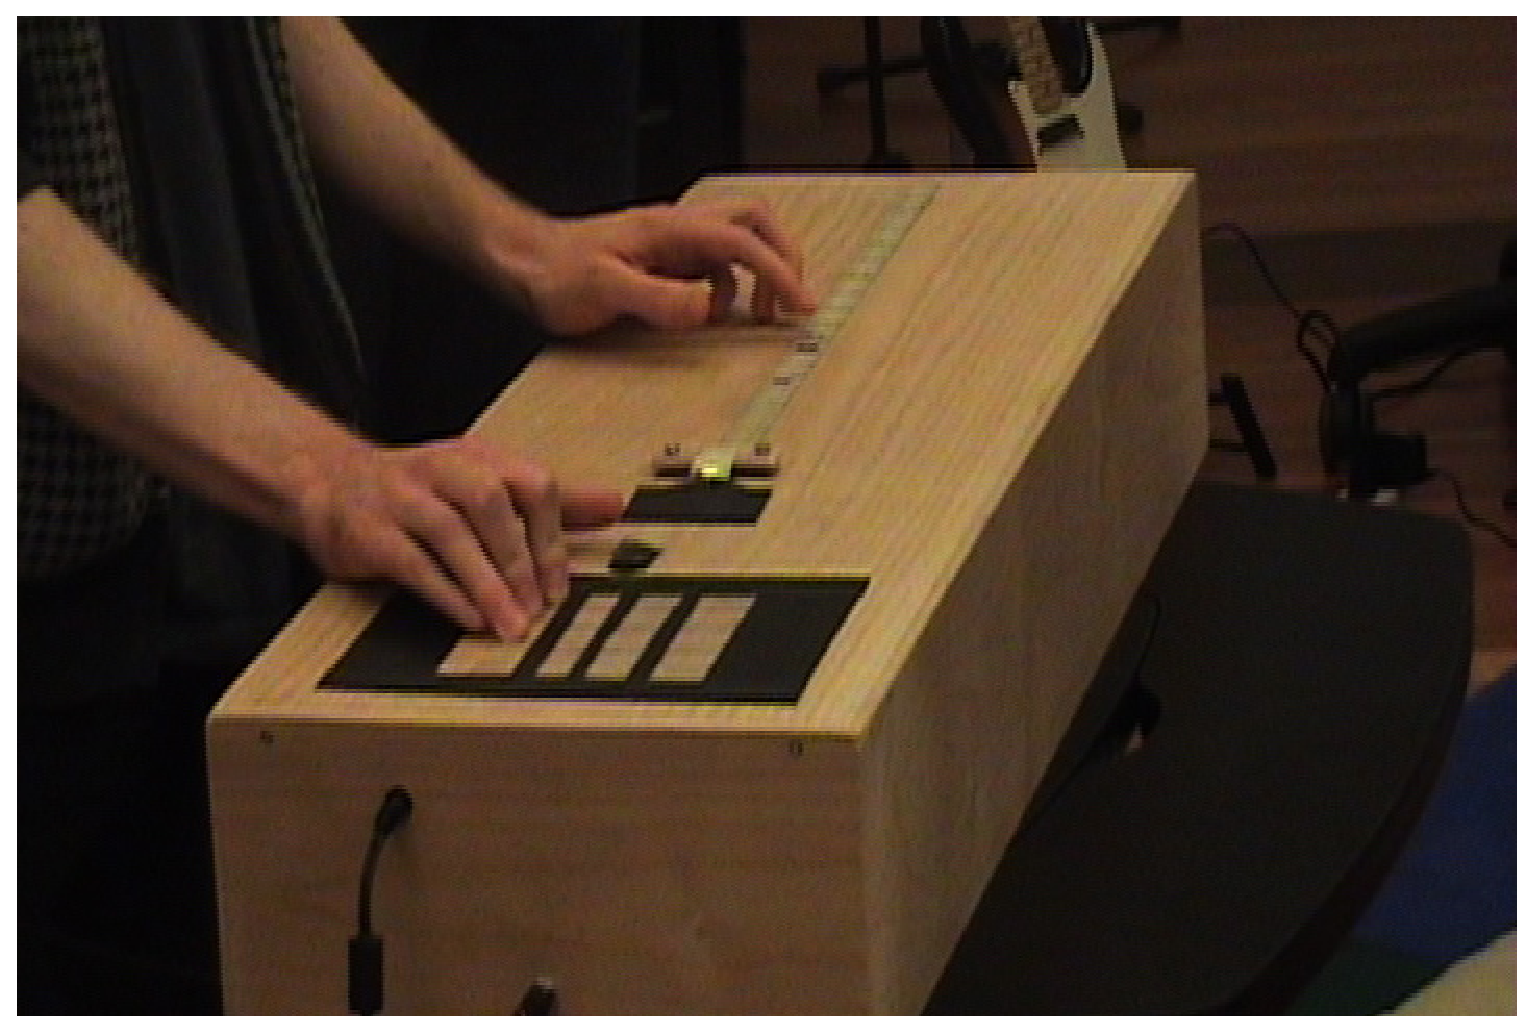
\includegraphics[height=1.55in, trim=20mm 0 50mm 0, clip ]{Photos/Quadrofeeliaperformance.eps}
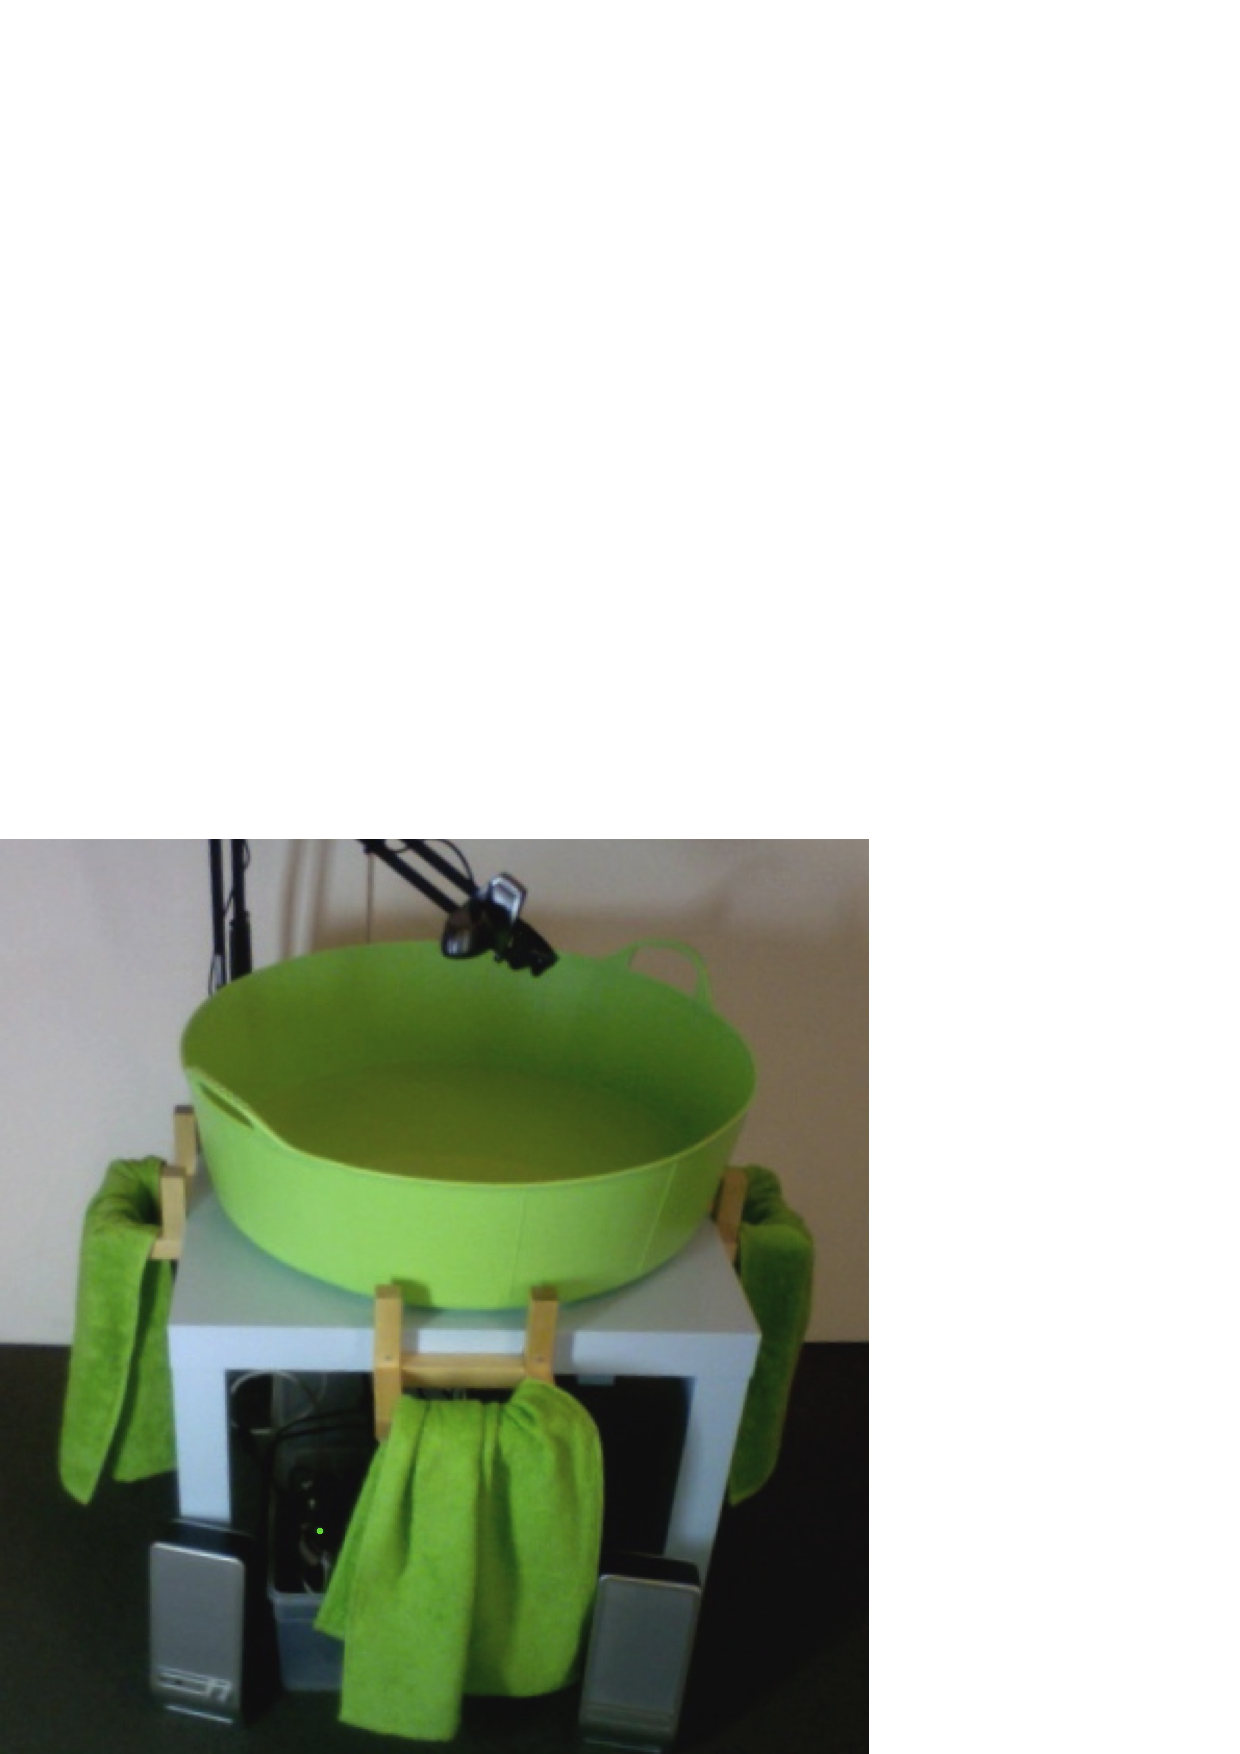
\includegraphics[height=1.55in]{Photos/Tuub.jpg}
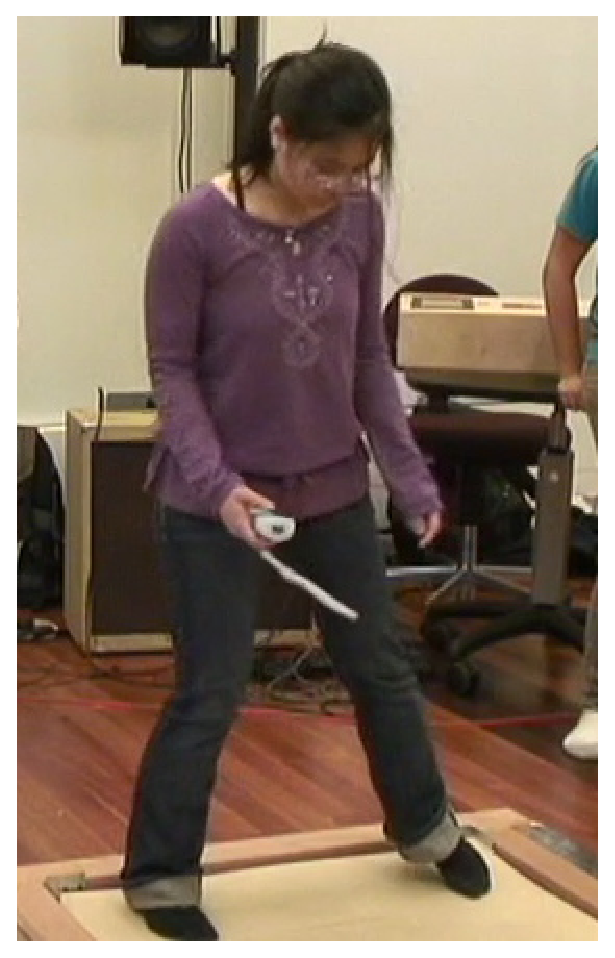
\includegraphics[height=1.55in]{Photos/DancePad3.eps}
	\caption {Some student projects made with Satellite CCRMA, from left: Quadrofeelia, Tub, Daft Datum.}
	\label{Berdahl:fig:studentprojects}
\end{figure}

\subsection{Independence/Autonomy}
One of our objectives in our design was to have the Satellite CCRMA platform be stand-alone. To this end, we set up the operating system so that it could boot reliably without a keyboard, mouse or monitor.  We strove to minimize the number of wires that needed to be connected to the system. We particularly focused on eliminating the need for the specialized cables that Beagle Board commonly use. Each additional cable or connector or AC adapter that had to be connected to the system at design or performance time was viewed as a liability, for the misplacement of any piece of the system is an obsolescence risk. Configured with battery power and lithium-ion powered speakers, it is possible to sense, synthesize and generate sound from just the Satellite itself.

We hope that the Satellite CCRMA platform will promote the development of long-lived projects by promoting independence of external systems.  This is why the platform incorporates both a microcontroller for sensing and a processor for synthesizing sound.  Although it is possible to connect Satellite CCRMA to the internet over either an Ethernet connection or wirelessly, we recommend that designers consider permanently disconnecting final projects from the Internet so that they are as independent as is practical.

\subsection{Native Floating Point Computation}

These projects require synthesis algorithms to synthesize the sound, but these can be computationally demanding.  Furthermore, although it is possible to implement most sound synthesis algorithms using integer computations or fixed-point computations, this process can be challenging and time consuming.  Indeed, David Zicarelli once quipped that he had heard that a programmer ``could either write fixed-point code or stay married.''  Such difficulties could distract students from design goals, forcing them to focus on specific engineering problems. Finally, many open-source libraries for synthesizing sound, such as Pure Data Extended, require floating-point computations.  For this reason, it was important that the Satellite CCRMA platform was capable of \emph{natively} carrying out \emph{floating-point computations}, as supported by the OMAP3530 processor.


\subsection{Compactness}
To promote flexibility and integration into other objects, the Satellite CCRMA is \emph{compact}. The Beagle Board itself has a 3"x3.5" footprint, and the Satellite CCRMA board fits into a 5.25"x7"x2" envelope, even with a generate breadboard for electronics onboard. This is small and light enough that it easily could be attached to a violin.  Small systems are easier to carry around, which meant that students were more likely to take their projects home to work on. The upcoming beta release of Satellite CCRMA will be even more compact as it is based on the Beagle Board xM with on-board Ethernet and USB support, so the GWC Technology HE2440 hub with Ethernet as shown beneath the Beagle Board in Figure~\ref{Berdahl:fig:Platform} will not longer be required. 

Only one of the projects in our course demanded a form factor too small for the Satellite CCRMA. In that project, the students made three tennis-ball sized balls that held Arduinos, a PIC-based sound synthesizer chip, a speaker and a battery. Looking forward, it would be an interesting challenge to see what the minimum size of the Satellite CCRMA platform could be while still using standard connectors. 

\subsection{Reconfigurability and Extensibility}
The open source and open hardware nature of Satellite CCRMA promotes \emph{reconfigurability} and \emph{extensibility}, which we found to be crucial to supporting the wide range of project ideas that our students had.  For us instructors, the fact that Linux drivers for Ubuntu were already available for a large number of external USB devices made it possible, for example, to quickly set up the Ethernet/USB hub and the Arduino for our students. For our students, it meant that they could add new hardware (such as bluetooth dongles, web cameras, and multi-channel audio devices) and new software (such as emacs, alpine, cwiid, jwm) with relative ease. 

The incorporation of the Arduino Nano and breadboard was also an important aspect to the Satellite CCRMA platform. To some degree, the Arduino was extraneous, because the Beagle Board's expansion port includes multiple serial interfaces and general-purpose I/O lines. However, we felt that it was very useful to be able to leverage our previous Arduino-based curriculum to help our students think about how to design interfaces and controls that were appropriate to the use, context, expression and metaphors they had selected. In the future, we will examine whether the extensibility offered by the Arduino over the native Beagle Board I/O is worth the foot print it takes up.

\begin{figure}[t]
	\centering
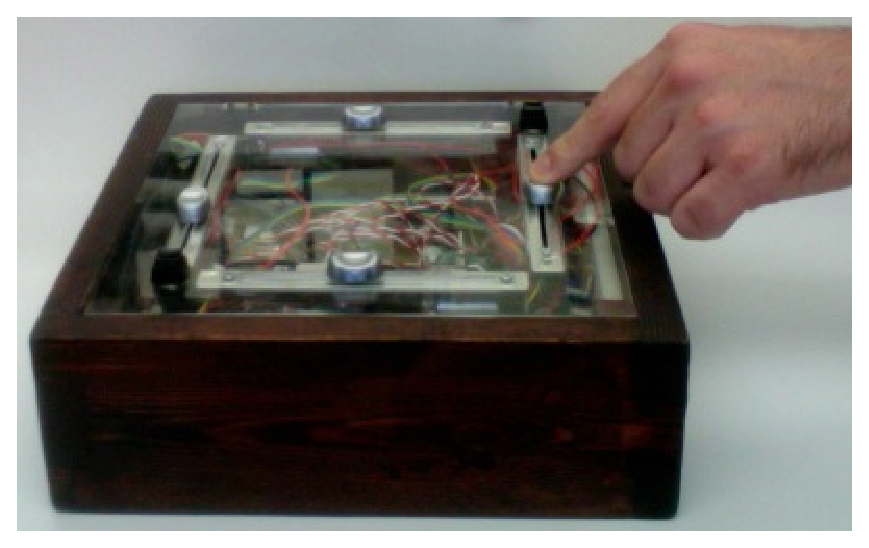
\includegraphics[height=1.35in]{Photos/SoundFlingerEd.eps}
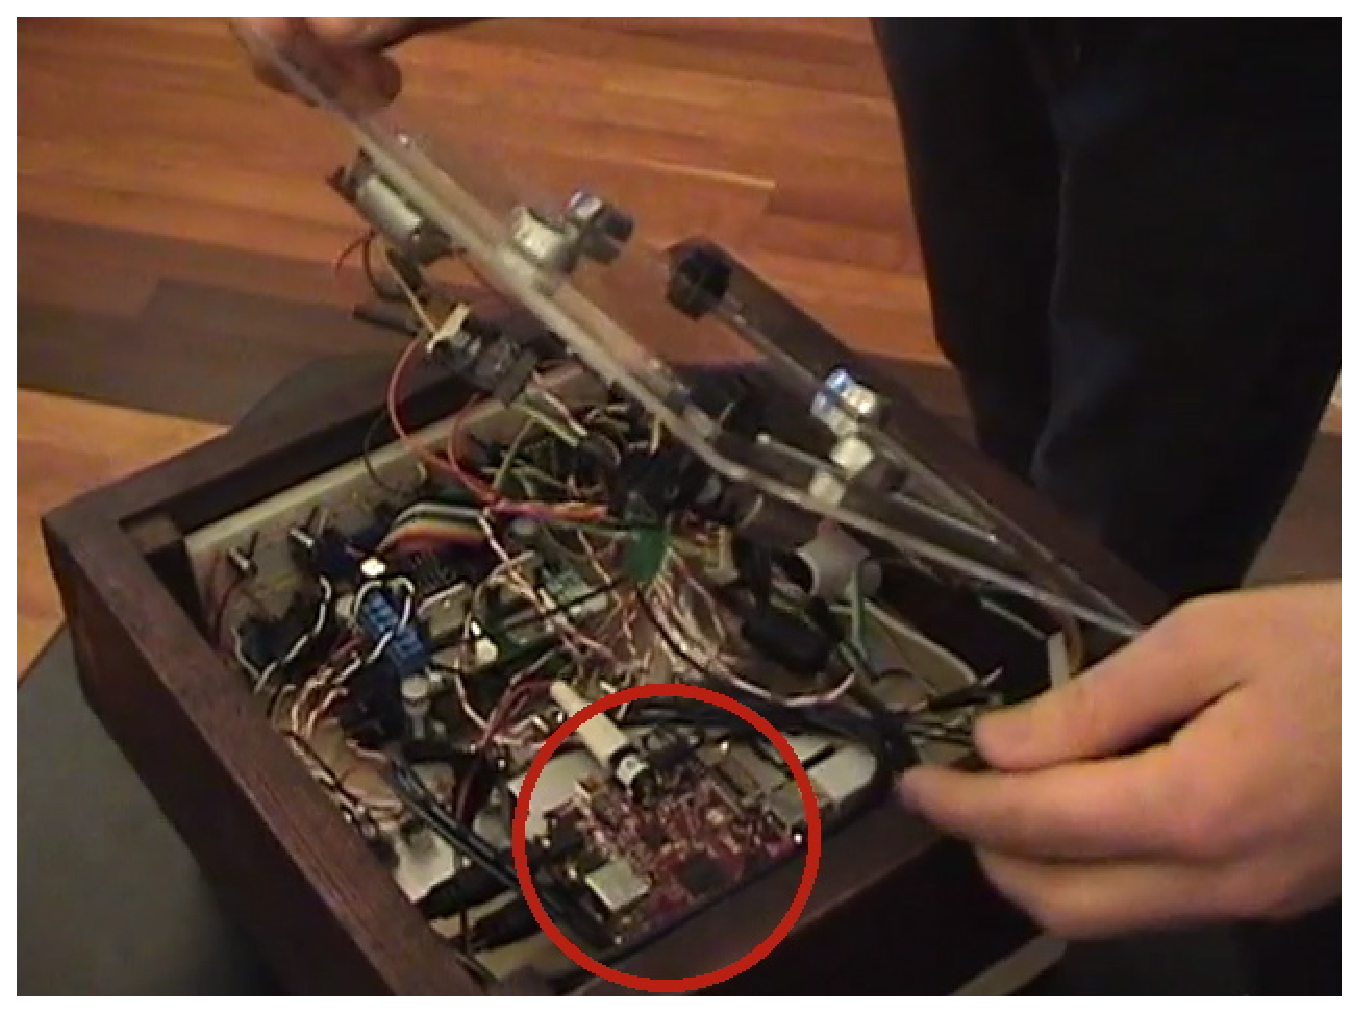
\includegraphics[height=1.35in]{Photos/SoundFlingerFlipOpen.eps}
	\caption{SoundFlinger}
	\label{Berdahl:fig:SoundFlinger}
\end{figure}

\subsection{Community support}

We previously mentioned how leveraging open source hardware and software made the Satellite CCRMA platform easy to reconfigure and extend. The open-source platform also makes it easier to develop a system of community support.  Beginning users can leverage examples so that they can get the platform up and running, while advanced users can find out how to tweak the system so that they have more control over the projects that they develop.  For example, the source code for any portion of the software can be obtained, modified, recompiled, and then loaded onto an SD card for use.  Similarly, the schematics and layouts for all of the core parts are available, enabling users to make custom boards based on the current state of the platform to meet any special needs.

Inspired by the community-based support and development efforts of platforms such as Processing \cite{Reas:2003} and Arduino \cite{Mellis:2007}, we have created a newsgroup aimed especially at artists to help address questions about the platform.\footnote{\url{http://groups.google.com/group/satelliteccrma}}. To help bootstrap the learning process, we provided our students with working code examples; these are available to other instructors, students or developers on the Satellite CCRMA site.

\section{Related Work}
\subsection{Prior platforms}
In the past, our course has been taught with platforms based on the Basic Stamp \cite{Verplank:2001}, the AVRmini \cite{Wilson:2003}, and the Arduino \cite{Mellis:2007}. Other past and current microcontroller-based platforms used for creating musical controllers include I-CubeX's Digitizer \cite{Mulder:1995}, STEIM's SensorLab and junXionboard, Microchip PIC-based Create USB interface \cite{Overholt:2006}, and CNMAT's uosc. All of these systems are meant to be interfaced with a computer, which receives data from the microcontroller (via serial, openSoundControl \cite{Wright:1997}, MIDI formats, for example) to synthesize sounds in software. While these systems all do an admirable job of translating physical phenomena from the real world to signals which can be translated to sound, they require the presence of a laptop or desktop computer to perform real-time sythesis of sound.

\subsection{Similar platforms}
Far fewer platforms are designed to replace the laptop or desktop computer in the physical interaction architecture. One notable platform is the Audiopint \cite{Merrill:2007} platform. The Audiopint, a 17cm x 17cm ``mini-itx'' VIA Epia EN1500 motherboard running Ubuntu Linux housed in a Pelican case, functions as a low-cost and flexible audio effects processor and syntehsizer. It uses Pure data \cite{Steiner:2005} to synthesize sound. Another platform is the Gluiph \cite{Kartadinata:2003}, which features Pure data running on a complex programmable logic device (CPLD). 

Satellite CCRMA builds on the ideas embodied by the Audiopint and Gluiph. The choice of the Texas Instruments' OMAP-based Beagle Board provides Satellite CCRMA with a small footprint (the Beagle Board itself is 3" wide x3.125" long x0.625" tall, and the platform footprint is 7" x 5.5"x2"), relatively low power consumption, and the potential for broader platform support from the wider OMAP and Beagle Board development community. The cost of Satellite CCRMA, critical to the cost-sensitive artists and musician community, is lower than either platform (\$125 at time of submission). Also, the use of a standard Linux operating system makes it easy to extend the system through opensource software and the use of USB-based computer peripherals and drivers available on-line. Finally, the incorporation the bread Board and Arduino helps to orient the use of the system towards the development of novel musical controllers and sound installations.

\subsection{Alternative Platforms}
One viable alternative to the Satellite CCRMA system is the use of low-cost netbooks in place of laptops. At the time of this paper's submission, low-end netbooks capable of running Pd cost ~\$300-\$400 USD. Although little has been published about the use of netbooks as musical system platforms, we believe it is only a matter of time before people start to dedicate inexpensive netbooks to their instruments. The catch is that, as small as netbooks are, the minimum size and layout of netbooks is dictated by typical laptop usage. Even though the cost of integrating features such as a screen, a lithium-ion battery and wifi and bluetooth capability to the Satellite CCRMA system would likely cost more than a similarly equipped netbook, the cost and difficulty of hacking and reconfiguring a netbook into a format that can be easily incorporated into an instrument would likely neutralize any potential savings.

Another alternative to using the laptop or desktop computer as a music platform is to use mobile phones or iPods. In earlier mobile music platforms, the phones were just used for their autonomous sensing capabilities, and an external PC was used to generate the sound, but more recently, sound synthesis on-the-phone has been pioneered using the Synthesis ToolKit on the Symbian OS \cite{Essl:2006b}, and the MoMu on the iPhone OS \cite{Bryan:2010}. The advent of the Android OS phones and tablets is likely to greatly decrease the cost of compact autonomous systems with the computational ability to generate sound, so that these devices will be cheap enough to dedicate to specific instrument or installation designs. However, it is fairly difficult as yet to interface external sensors with these systems, which greatly limits the range of musical control and interaction capabilities of platforms based on these systems. Most strategies involve using Bluetooth wireless, which introduces some latency due to the Bluetooth protocol.

\begin{figure}[t]
\centering
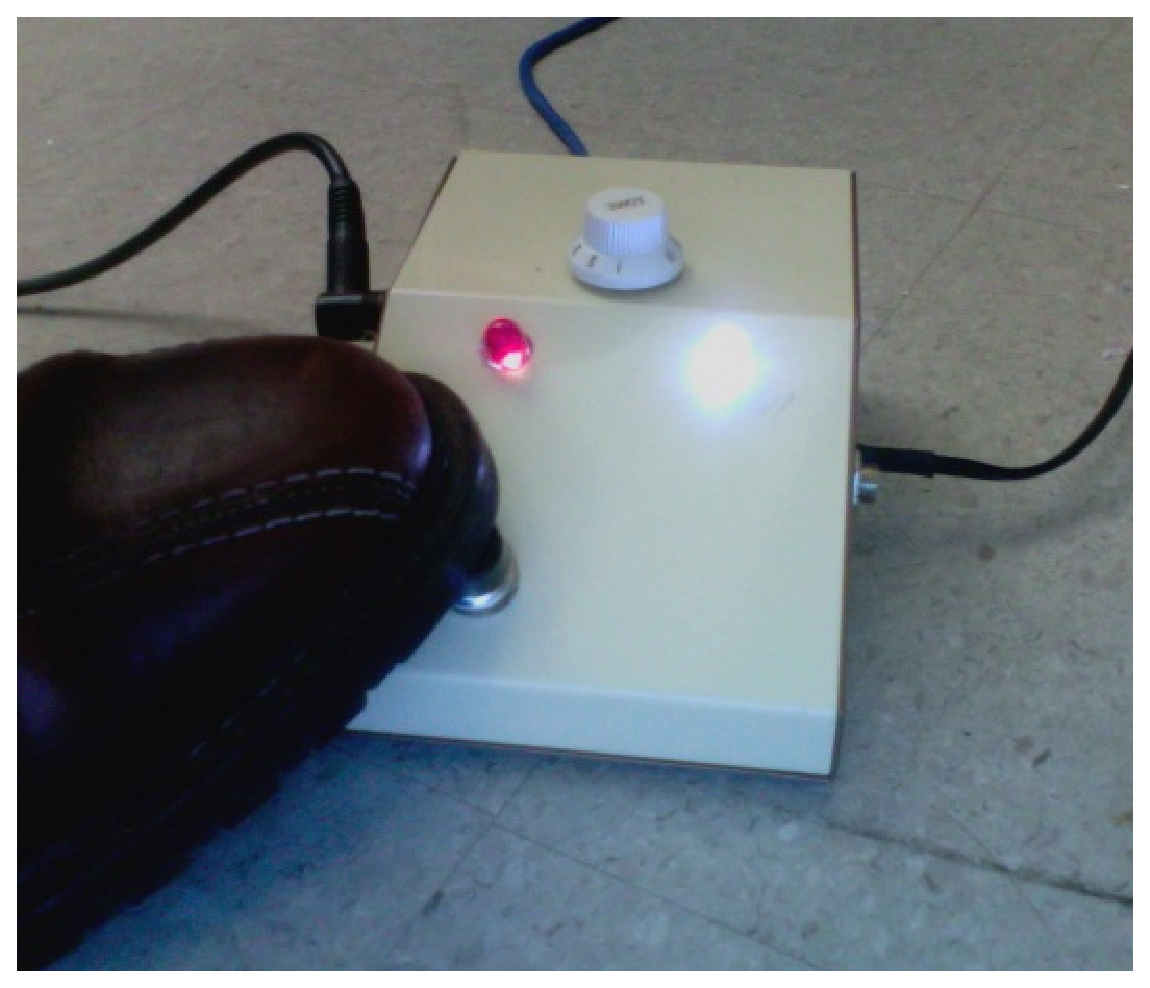
\includegraphics[height=1.5in]{Photos/Stompbox.eps}
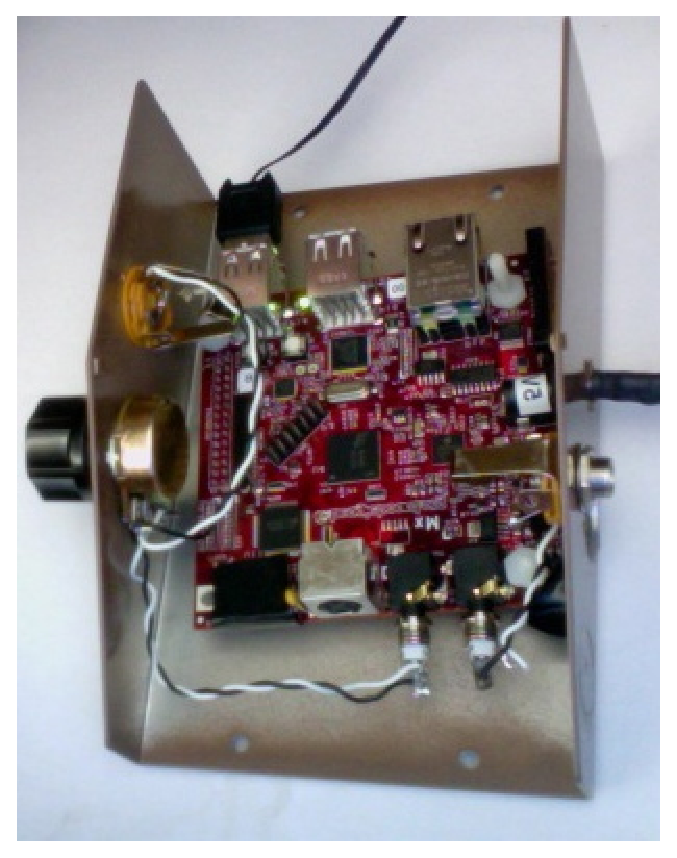
\includegraphics[height=1.5in]{Photos/BottomFxPedal.eps}
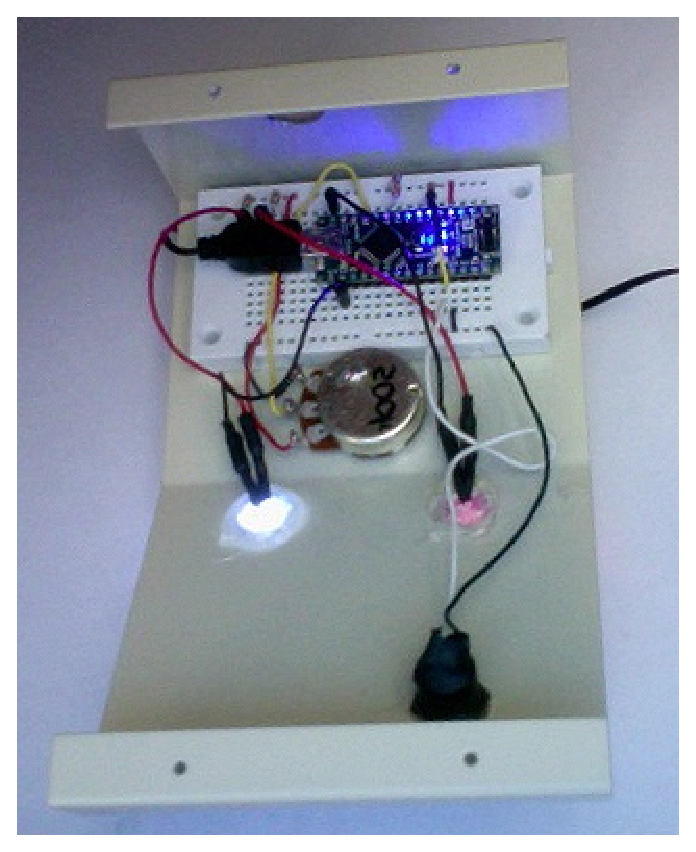
\includegraphics[height=1.5in]{Photos/TopFxPedal.eps}
\caption{Example Stompbox featuring Beagle Board-xM}
\label{Berdahl:fig:Stomp}
\end{figure}

\section{Project Highlights}
To illustrate the range of what is can easily be accomplished with Satellite CCRMA as a platform, we present these examples of what our students created for the class projects. Many of the students were new to the Arduino when they started the class, and all of the students were new to the Beagle Board and embedded Linux.

\subsection{Independent Musical Instrument}
Quadrofeelia, by Jiffer Harriman, Mike Repper, Linden Melvin, and Locky Casey, (see Figure~\ref{Berdahl:fig:studentprojects}) shows that Satellite CCRMA can be employed to construct an \emph{independent} musical instrument that does not require connections to any external computers.  A musician plugs the 5V power supply into a wall outlet, and then the 1/4'' audio output jack produces an output signal that can be connected to a guitar amplifier or public address system.  As the musician manipulates the sensors embedded in the instrument, output sound is produced in response.  Quadrofeelia bears resemblance to a slide guitar, but with more abilities for retuning the chord tunings and inversions due to the buttons manipulated by the right hand.
%\subsection{Force-Feedback Control}

\subsection{Independent Dance Interface}
Standard sensing devices typically employed for gaming are incorporated into Daft Datum, a musical instrument played by the feet, by Rosie Cima, Ravi Kondapalli, and Ben-Zhen Sung.  A dance pad is hidden beneath the performer's feet and sends data to Pure Data over USB using the \texttt{hid} object.  To discover the vendor and product IDs for the dance pad, the \texttt{dmesg} command can be executed in Linux directly after plugging in the dance pad.  No further configuration is necessary.  To change the sound synthesis mode, the performer presses buttons on the Wiimote as shown in Figure~\ref{Berdahl:fig:studentprojects}.  The Wiimote communicates with Pure Data over a remarkably small Wifi USB dongle that can be setup as described on the Wiki.\footnote{
\url{https://ccrma.stanford.edu/wiki/Making_a_Wii_remote_talk_to_Pure_Data_(PD)}}



\subsection{Video-based Interactive Installation}
The T\"ub,  by Marc Evans, Bj\"orn Erlach, and Mike Wilson, demonstrates the video capabilities of Satellite CCRMA.  The KWC-1301 USB Webcam is supended above a tub of water (see Figure~\ref{Berdahl:fig:studentprojects}, top center) and transmits images to Pure Data running on the Beagle Board stored underneath the tub.  Objects in Pure Data's Graphics Environment for Multimedia (GEM) generate sound samples by scanning along circles in the images.  If the water is still, then there is almost no sound, but waves in the water create buzzing sounds, whose timbre evolves with the wave motion.  Installation visitors can induce waves in the water using a variety of techniques: poking the water with their hands, pulling the edge of the tub with their hands, poking the water with tubes, blowing water through tubes, etc.



\subsection{Multichannel Audio in a Collaborative Installation Piece}
The Sound Flinger, by Chris Carlson, Hunter McCurry, and Eli Marschner, demonstrates that Satellite CCRMA is compatible with an external sound interface.  The device, as shown in Figure~\ref{Berdahl:fig:SoundFlinger}, allows users to play back snippets of live recorded sounds through four output audio channels provided by the SIIG IC-710112 USB Soundwave 7.1 Digital audio adapter, which is placed underneath the Beagle Board circled in red in Figure~\ref{Berdahl:fig:SoundFlinger}.




\subsection{Audio Effects Stompboxes}
Because Satellite CCRMA incorporates audio codecs and native floating-point computation, implementing digital audio effects is relatively straight-forward even for novices.  The design history of audio effects incorporates a rich past of audio effects controlled primarily by knobs, switches, and even sometimes pedals.  Figures \ref{Berdahl:fig:Stomp} and \ref{Berdahl:fig:Stomp} (left) show an example \emph{stompbox}, which incorporates a footswitch and two extra large LEDs.  The stompbox demonstrates that Satellite CCRMA can also be employed for teaching audio digital signal processing (DSP) in an embedded systems context.  Appropriate languages for DSP include Faust, C++, Pure Data, ChucK, etc.


\section{Satellite CCRMA Website}
The main website for the project\footnote{\url{https://ccrma.stanford.edu/satellite/}} provides links to videos of project presentations, the Satellite CCRMA newsgroup, Wiki, and SD card images.


\section{Future}
Since the beginning of this project, we have already had one major hardware change, from the OMAP 3530-based Beagle Board to the OMAP 3730-based Beagle Board-xM. While we believe the OMAP-based Beagle Board family to be a promising platform for the design of new interfaces for musical expression, the core aim of the Satellite CCRMA project is to develop standalone computational capabilities for musical interfaces in an open-source setting. As such, we are tracking related platforms such as the Hawk Board, Panda Board, Crane Board, or GumStix, in case any of these should become more viable for our project goals. In any case, it is our intent to maintain a similar set up of core platform software across hardware changes, and also to make migration from one platform to the next graceful for users. 

We have found that the existing platform is stable and easy enough for NIME students to use, reconfigure and extend within the confines of a single school term. In the future, we hope to see if the Satellite platform helps promising projects grow beyond their short-term novelty ''stunt'' phase to become more mature musical instruments. In particular,  we hope to see whether inventors develop more expertise with their designed installations and instruments, perhaps by making more refinements, developing greater expertise in playing their instrument, or by making scores for the systems' unique capabilities.  We also intend to perform more detailed analysis to see if the Satellite CCRMA system helps students to more fully understand full-scale system design.

\section{Conclusions}
In conclusion, we found that the introduction of the Satellite CCRMA platform has provided our students with a more full-featured, robust and flexible system for lab exercises and musical interaction design projects. This platform extends the portability, scalability and support community of our previous microcontroller-based system to the microprocessor as well. We have found the platform is useful for instrument-based and installation-based systems, and we are actively promoting the platform to see if it is useful in a wide variety of other applications as well. 


\begin{acknowledgement}
In addition to Chris Chafe, Fernando Lopez-Lezcano, Bill Verplank, Max Mathews, Perry Cook, Julius Smith III, Michael Gurevich, Carr Wilkerson, and the open-source community, we would like to thank our students who helped us test the initial release of Satellite CCRMA: Chris Carlson, Locky Casey, Roseann Cima, Bj\"orn Erlach, Marc Evans, Francesco Georg, Jiffer Harriman, Ravi Kondapalli, Eli Marschner, Hunter McCurry, Linden Melvin, Michael Repper, Mike Rotondo, Spencer Salazar, Ben-Zhen Sung, and Mike Wilson. This research was made possible by a generous equipment donation from Texas Instruments.
\end{acknowledgement}


\section*{Author Commentary: Satellite CCRMA for Embedded Musical Instruments and Embedded Sound Art}

\paragraph{Edgar Berdahl and Wendy Ju}

Our original motivation for creating Satellite CCRMA was to make a great platform for students to use in our NIME class.
We were particularly inspired by Wilson et al's 2003 paper \textit{Microcontrollers in Music HCI Instruction} \cite{Wilson:2003},
which described the Atmel-based platform that preceded the Arduino \cite{Banzi:2009}. At the time, the platform was state-of-the-art,
with an Atmel chip interfacing with sensors and conveying sensor data over a cable to a desktop computer for
synthesizing sound. However, by 2011, we felt that moving to a modern, self-contained, embedded, single-board Linux
computer could reduce obsolescence and bolster reliability and mastery in NIME instruments. There are reports of
still-functional versions of the instruments created by students---Jiffer Harriman said of the \textit{Quadrofeelia}
from 2011, ``I've pulled it out to demo with a group of kids recently but it mostly sits on a shelf.'' Even that feels like a triumph.

Overall a large number of community members have engaged with
Satellite CCRMA. Besides the workshops that we have taught, the online discussion group has grown to 217 members.
Since the group messages can be viewed by anyone online, most likely many more people have made use of the messages on
the group. This facilitates the creation of projects in laboratories across the world.
A few select external projects include Roberto Morales'
\textit{Zanate de Luz}, Scott Smallwood's \textit{Sync or Swim II}, Time's Up's \textit{Mind The Map}, Martin
Hünninger's \textit{Guitar-Granulator}, Ulysse Rosselet's \textit{Music Box}, soccer-playing sonic robots by Ralf Hoyer
with Andre Bartetzki, and more.\footnote{\textrm{ See the Satellite CCRMA project page at
}\url{https://ccrma.stanford.edu/~eberdahl/Satellite/}\textrm{ which includes links to media examples as well as a link
to the discussion group.}} The most amazing thing, though, for
both of us, is to meet people who tell us about embedded instruments they have made using Satellite CCRMA without
knowing that we had anything to do with it---so on that level we can feel the impact of this work.

In our original paper, we discussed competitors and alternatives to Satellite CCRMA---issues we brooded long and hard
over during the development. Originally, Satellite CCRMA was supported for the Beagle Board and Beagle Board xM boards.
These were some of the earliest DIY-oriented embedded Linux boards that were capable of natively computing audio using
floating-point hardware. Later, the Raspberry Pi board emerged as a lower-cost alternative. For this reason, Satellite
CCRMA has been migrated to the Raspberry Pi \cite{Berdahl:2013}. Despite the trade-off in audio quality, that made for a more
attractive platform globally. Indeed, to date over 5 million Raspberry Pi boards have been sold, indicating a large
number of potential users. The various audio needs of users can be met according to scale: beginning users can use
on-board audio, more advanced users can improve the audio quality by attaching a small USB audio dongle, and
researchers can attain eight-channel audio output by employing a larger USB audio device.

In September 2014, a new Satellite CCRMA image was made available for the Raspberry Pi~2. It provides an order of
magnitude increase in computational power for audio DSP, largely due to architectural improvements in the (now
multiple) ARM Cortex-A9 cores. With this, the Satellite CCRMA project is in our opinion coming of age in the sense that
users now no longer need to be as careful to write efficient audio programs. Instead, users can focus more on employing
more preferred programming techniques to create desired audio programs. This suggests that in the coming years, it will
become even easier for students to successfully realize fully functional and beautiful embedded musical instruments and
embedded sound art.

As we look toward the future, Edgar Berdahl's new research group has focused on designing \textit{embedded acoustic
instruments}. These are embedded musical instruments that incorporate sensors, self-contained audio DSP, and an
internal mechanism for radiating sound \cite{Berdahl:2014}. They are like traditional acoustic instruments in that the radiated sound
comes from a location close to the sensors, and performers feel the sonic vibrations throughout the instrument body.
This technology has been demonstrated using instruments such as the\textit{ Stingray}, \textit{LapBox} and
\textit{Textural Crossfader}.

Satellite CCRMA also points to uses for inexpensive lightweight development platforms in applications beyond music.
Wendy Ju's new research group has been developing an Interaction Engine inspired by Satellite CCRMA that is targeted
for human-robot interaction and making interactive devices---the tools on that platform are targeted at motor control,
remote messaging and remote access to sensors \cite{Martelaro:2016}. From that perspective, computer music is a forerunner for a wider
array of interactive and expressive products in the age of the Internet of Things.






\section*{Expert Commentary: Towards a community standard for self-contained instruments}

\paragraph{Andrew McPherson}


In this paper, Berdahl and Ju highlight a persistent problem facing the NIME community: the short lifespan of most digital musical instruments. Though some of the causes are human rather than technical, making a digital instrument that still works many years later turns out to be pretty hard. Using a general-purpose computer means that future OS or software updates could break the instrument. Custom hardware designs face a different set of problems: parts become obsolete and hard to find, or insufficient documentation during the initial design means that maintaining the instrument later requires tedious reverse engineering.

Perhaps NIME needs a sort of ``digital musical instrument archive'': a repository coupled to a hardware/software platform which is consistently maintained and documented, reasonably standardised across the whole community, and where instruments can be maintained in near perpetuity by staying locked to particular versions of any underlying tools. Whether such an archive could exist and cover the full breadth of NIME activity is uncertain, but if it ever happens, Satellite CCRMA may well be where it starts.

Hardware prototyping toolkits for interactive systems have been around for many years (see for example Mulder's I-Cube system in the 1990's \cite{Mulder:1995}). The big change in past 5 years has been that, driven by the mobile phone market, low-power embedded processors have finally started to catch up to laptops in terms of real-time audio processing capability. That means that platforms which previously could only gather sensor data for a computer can now handle the complete operation of an instrument.

Satellite CCRMA is, in essence, a laptop replacement. Established music software such as Pd and ChucK run on an embedded ARM computer (originally a BeagleBoard, now a Raspberry Pi 2), which in turn connects to an Arduino for hardware I/O. The beauty of it is that the tools are familiar from laptop music-making, but the device can operate independently of the computer. The hardware cost is much reduced without the computer, so it becomes feasible to keep the instrument intact indefinitely.

Berdahl and Ju write: ``it will be many years before we can empirically determine whether our platform is indeed longer-lived than the alternatives.'' It has only been 4 years, but the initial evidence is promising, in large part because of their active maintenance of the platform, updating it for the latest single-board computers and the latest software versions. Projects using Satellite CCRMA have appeared on YouTube and high-readership sites like Create Digital Music \cite{Barreiro:2013}. It both benefits from, and contributes back to, the existing open-source communities around the tools it builds on (Arduino, Raspberry Pi, Pd etc.).

A still-open question is whether there can, or indeed should, be one single platform which unifies the needs of all DMI designers. The risks of fragmentation are clear: when every designer has their own toolset, the benefits of sharing and interoperability are lost. But the technical needs of digital instruments may be as diverse as the music they create.

The weak link in the laptop-based instrument is typically the coupling between the sensors and the sound generator. In particular, USB-to-serial connections to Arduino suffer from bandwidth limitations and (even on the newer native-USB boards such as the Leonardo) unpredictable latency and jitter from the host system's USB drivers. A secondary limitation, affecting embedded devices more than laptops, is that high-level music languages are not always the most CPU efficient, which can translate to larger buffer sizes and increased latency.

Satellite CCRMA, as a modular system, inherits some of these standard issues (for now). But in exchange, it gains the benefit that the tools are familiar, and that each tool can be reconfigured independently. As embedded hardware power continues to increase, spending a few CPU cycles to save days or weeks of engineering time looks like an increasingly good trade.

Satellite CCRMA was one of the inspirations for my own BeagleRT embedded audio/sensor platform \cite{McPherson:2015}, and a literature search shows it has inspired other designers as well. Its influence is no surprise. Making a common platform suitable for self-contained musical instruments is an appealing goal with a long history, and other designers can learn a lot from Berdahl's and Ju's specific approach. The combination of familiar open-source software, regular updates, teaching and community building has created a versatile tool which appeals to musicians and engineers alike. 

